\section{Результаты}

\subsection{Гистограмма и график плотности распределения}


\begin{figure}[H]
	\begin{tabular}{ccc}
		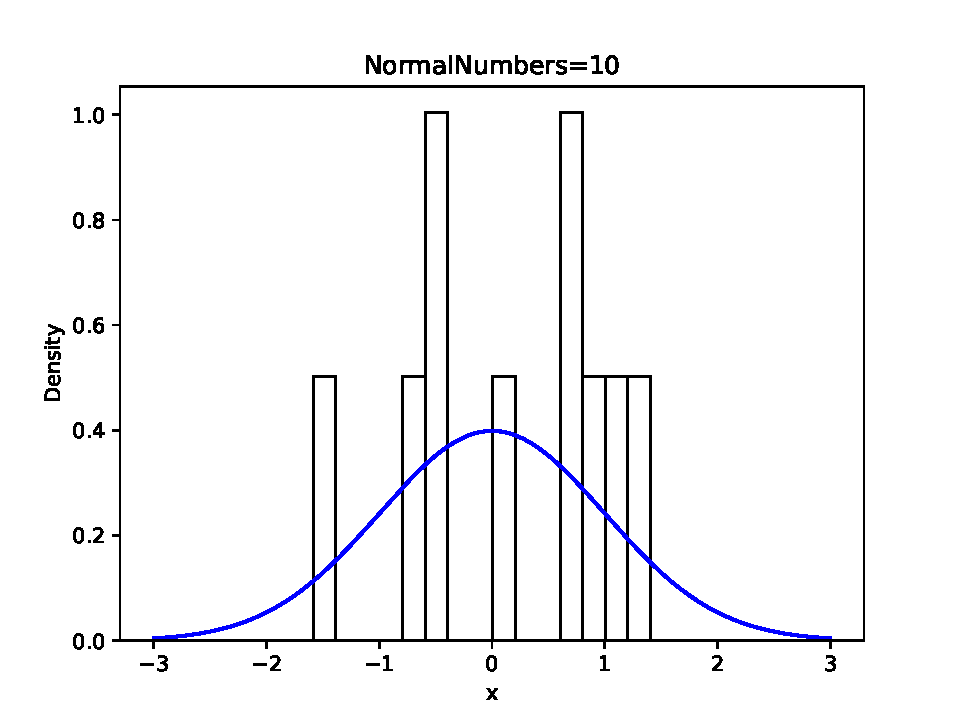
\includegraphics[scale=0.33]{normal_hist_10.pdf}
		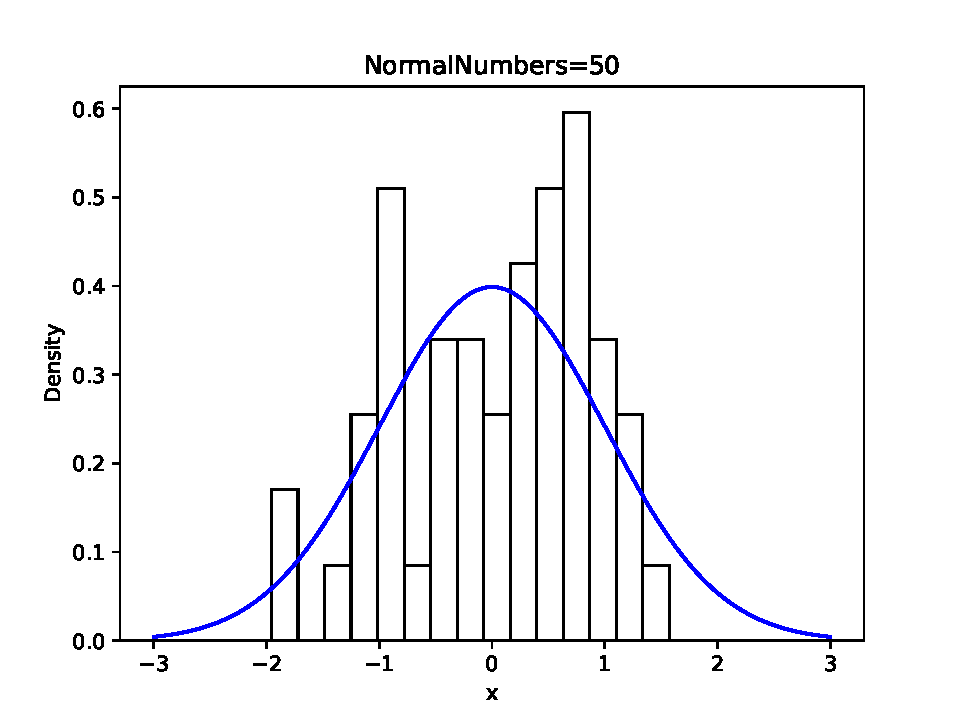
\includegraphics[scale=0.33]{normal_hist_50.pdf}
		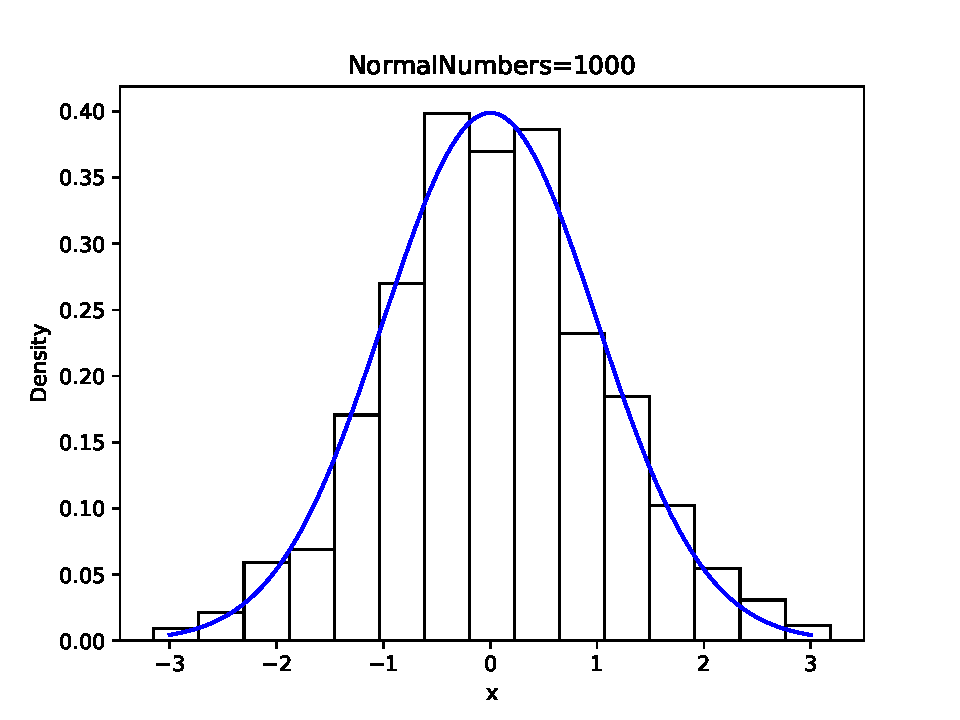
\includegraphics[scale=0.33]{normal_hist_1000.pdf}
	\end{tabular}
	\caption{Нормальное распределение}
\end{figure}

\begin{figure}[H]
	\begin{tabular}{ccc}
		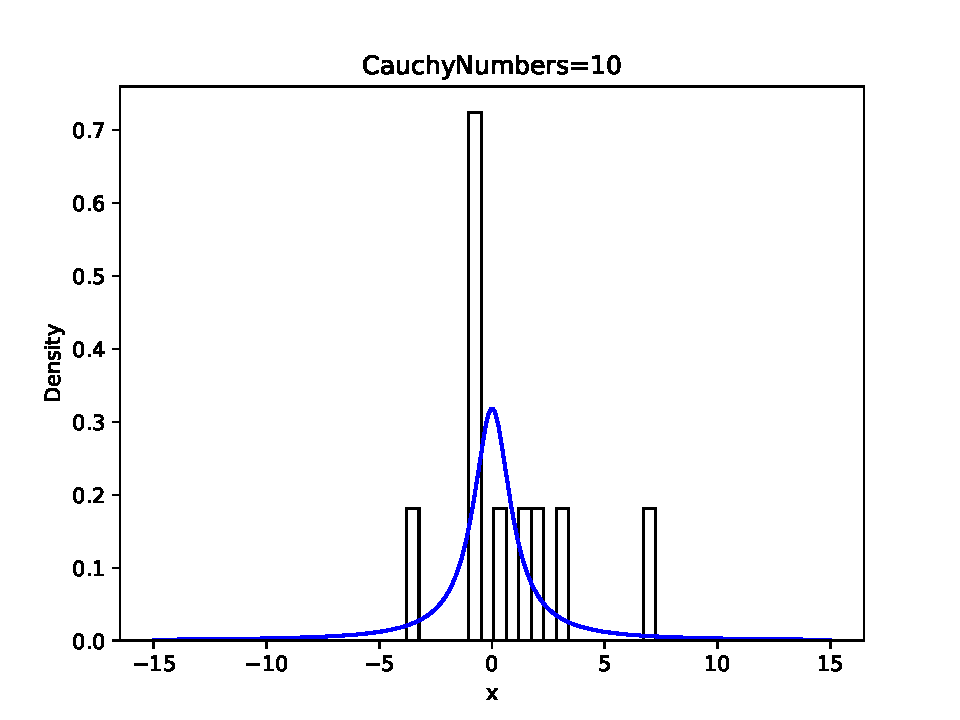
\includegraphics[scale=0.33]{cauchy_hist_10.pdf}
		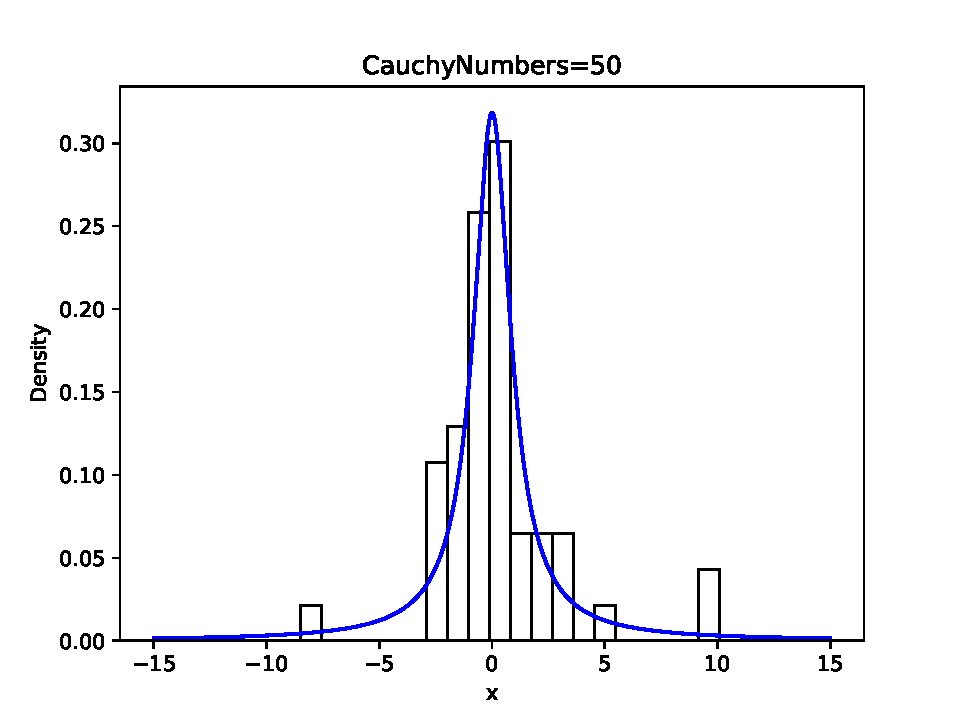
\includegraphics[scale=0.33]{cauchy_hist_50.pdf}
		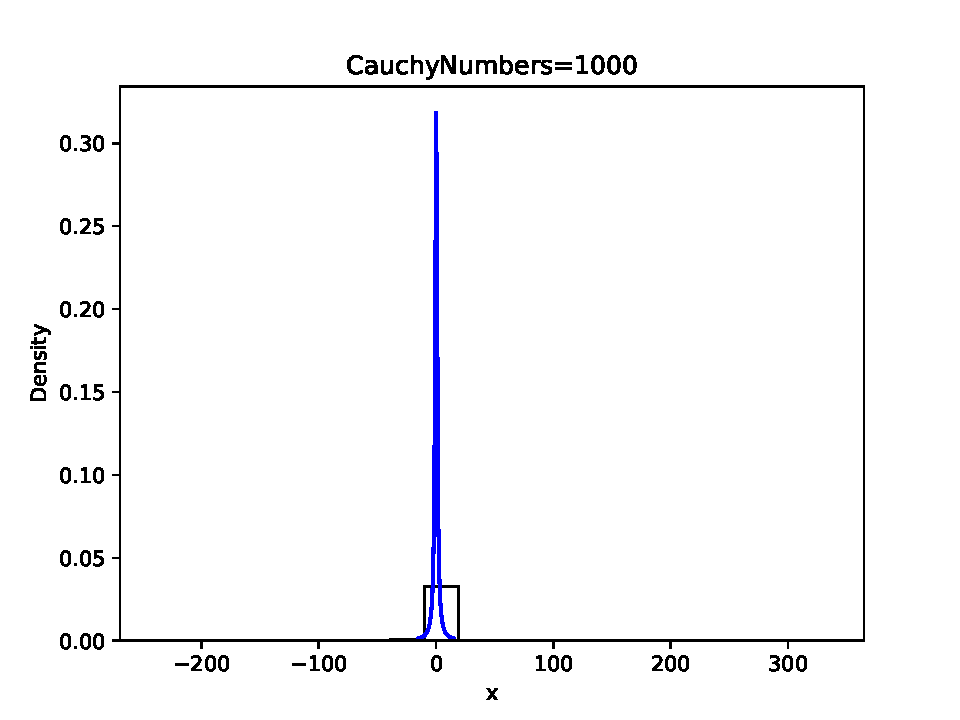
\includegraphics[scale=0.33]{cauchy_hist_1000.pdf}
	\end{tabular}
	\caption{Распределение Коши}
\end{figure}

\begin{figure}[H]
	\begin{tabular}{ccc}
		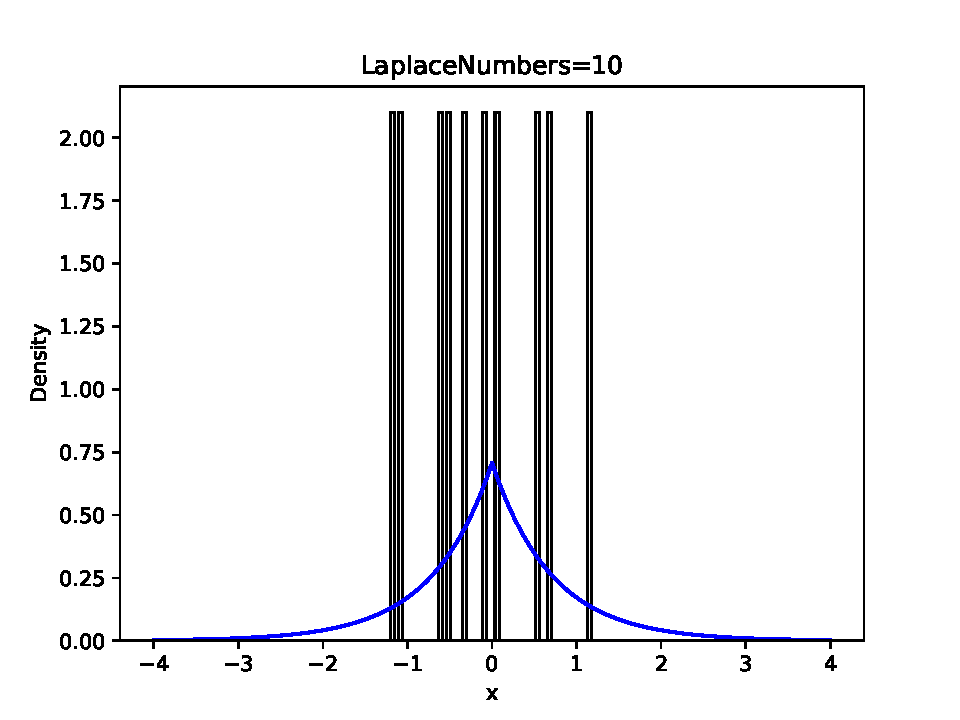
\includegraphics[scale=0.33]{laplace_hist_10.pdf}
		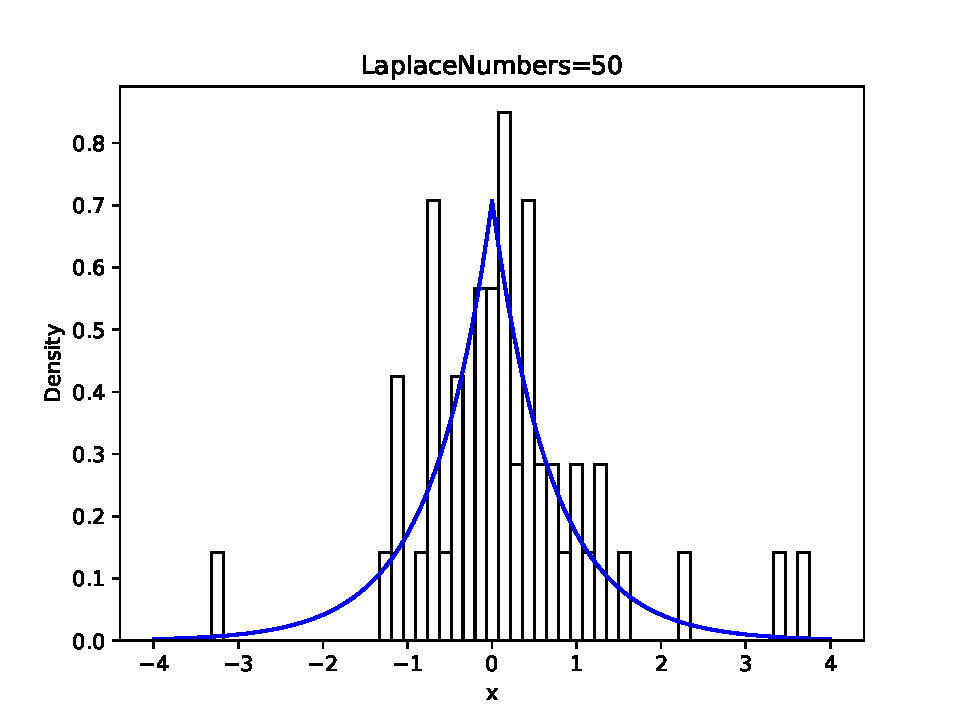
\includegraphics[scale=0.33]{laplace_hist_50.pdf}
		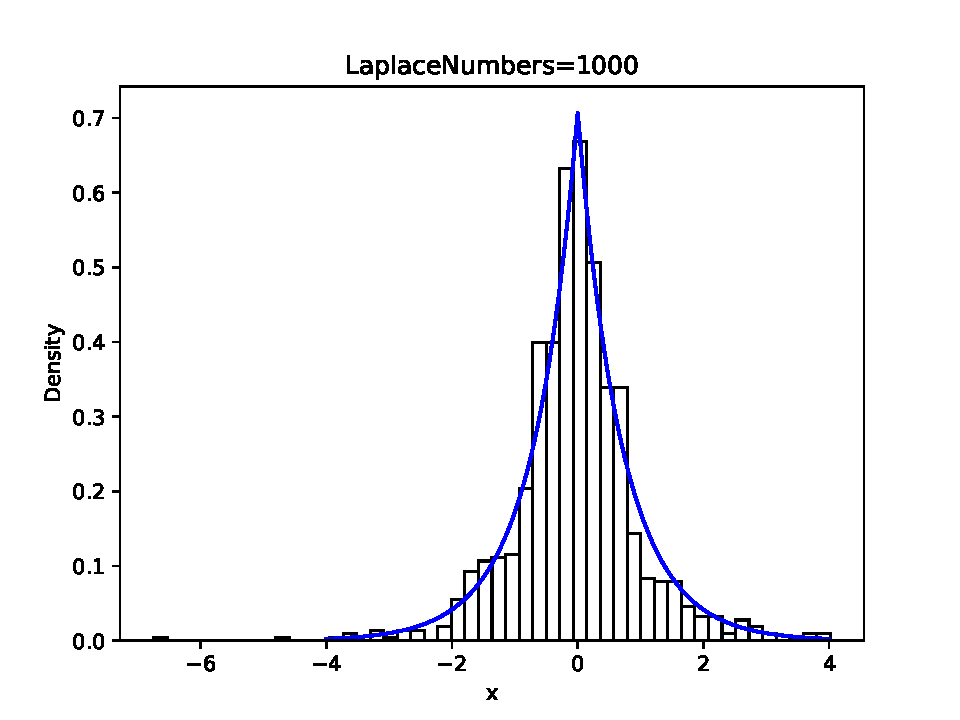
\includegraphics[scale=0.33]{laplace_hist_1000.pdf}
	\end{tabular}
	\caption{Распределение Лапласа}
\end{figure}

\begin{figure}[H]
	\begin{tabular}{ccc}
		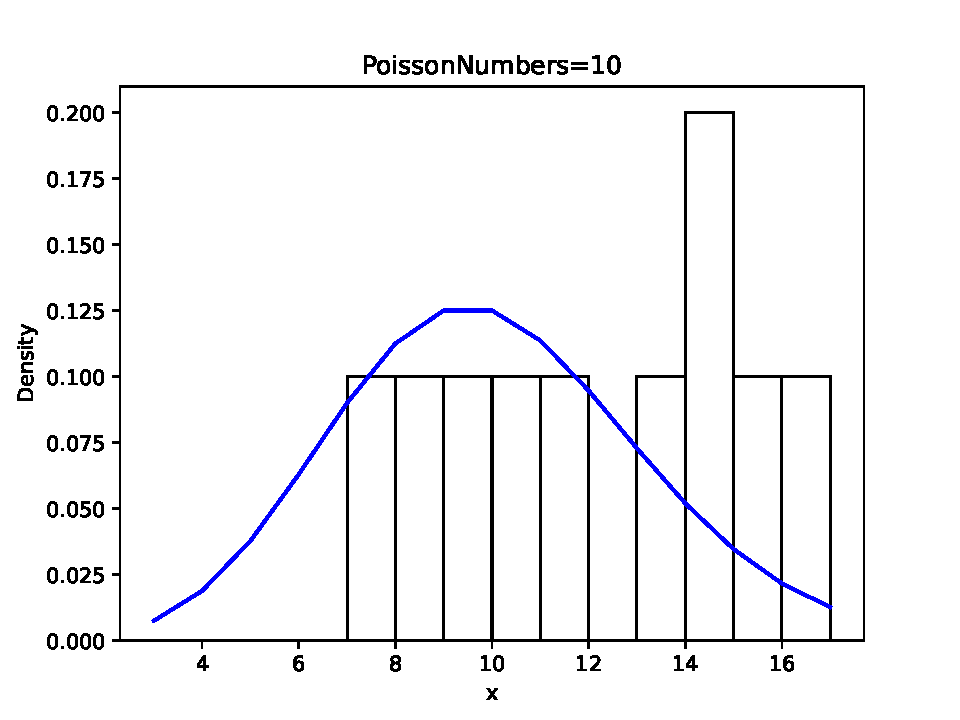
\includegraphics[scale=0.33]{poisson_hist_10.pdf}
		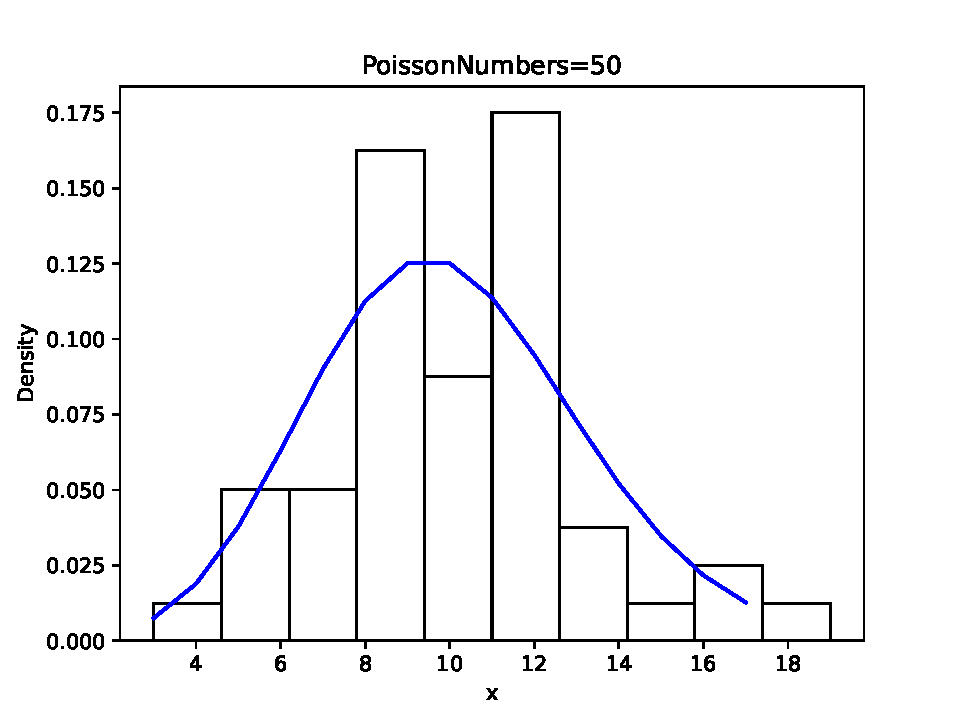
\includegraphics[scale=0.33]{poisson_hist_50.pdf}
		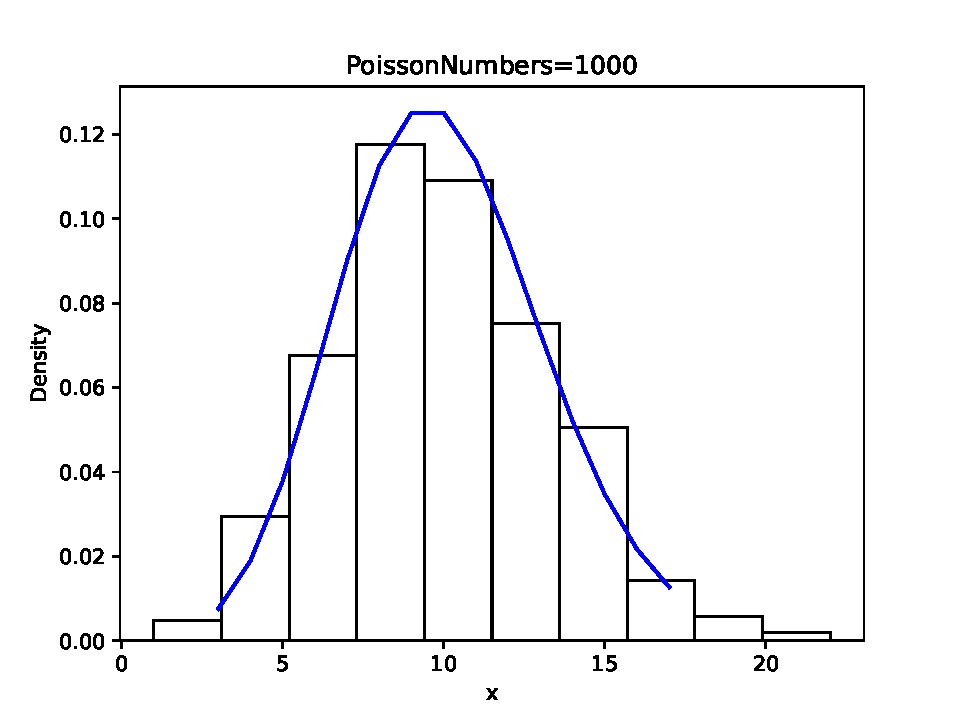
\includegraphics[scale=0.33]{poisson_hist_1000.pdf}
	\end{tabular}
	\caption{Распределение Пуассона}
\end{figure}


\begin{figure}[H]
	\begin{tabular}{ccc}
		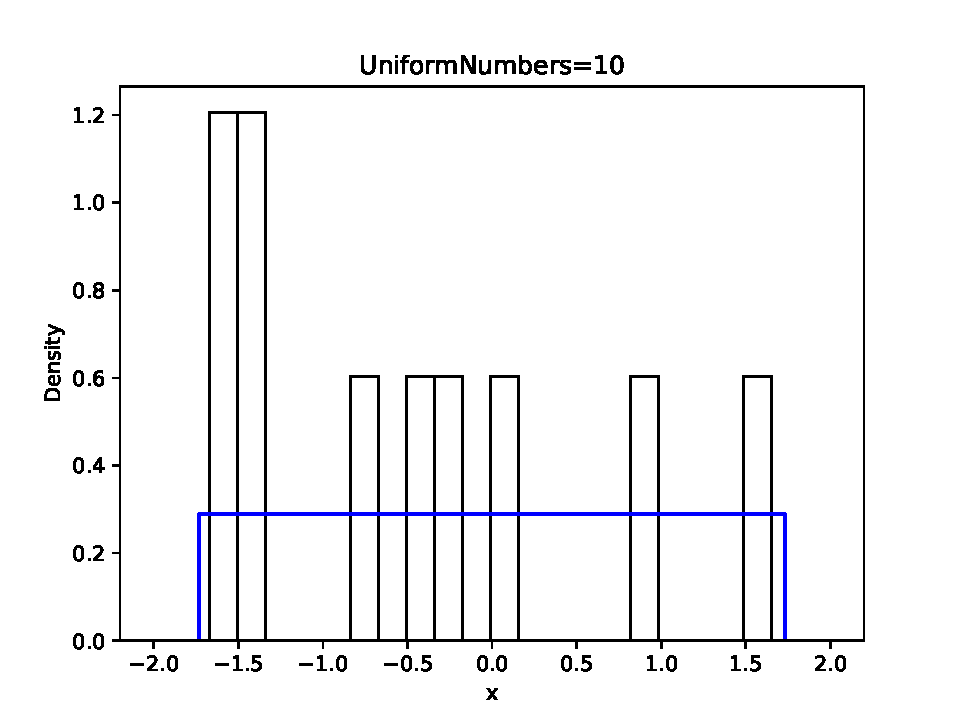
\includegraphics[scale=0.33]{uniform_hist_10.pdf}
		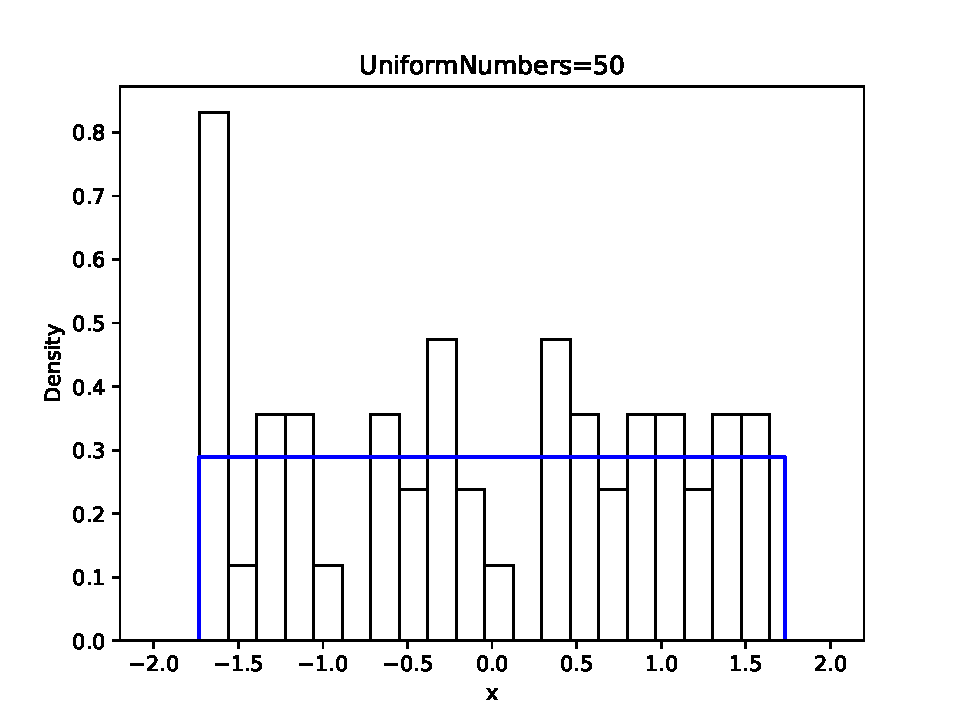
\includegraphics[scale=0.33]{uniform_hist_50.pdf}
		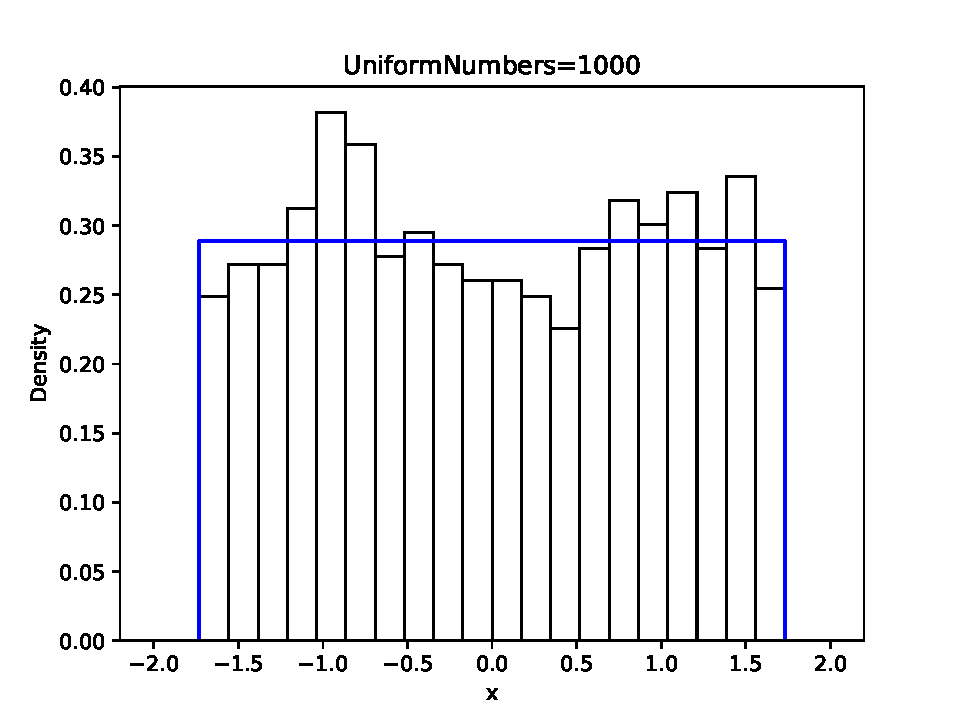
\includegraphics[scale=0.33]{uniform_hist_1000.pdf}
	\end{tabular}
	\caption{Равномерное распределение}
\end{figure}


\subsection{Характеристики положения и рассеяния}

Округление проводилось следующим образом: 

В оценке $x = E \pm D$ вариации подлежит первая цифра после точки. В данном случае $x = 0.0 \pm 0.1k$, \\
k зависит от доверительной вероятности и вида распределения (рассматривается в дальнейшем цикле лабораторных работ).\\
Округление сделано для $k=1$
 

\begin{table}[H]
	\begin{center}
		\begin{tabular}{|c||c|c|c|c|c|}
			\hline
			Normal n=10 & $\overline{x} $ & $med\:x$ & $z_{R}$ & $z_{Q}$ & $z_{tr}$ \\
			\hline\hline
			$E(z)$ & -0.00423 & 0.00676 & -0.01363 & -0.00839 & 0.00216 \\
			\hline
			$D(z)$ & 0.09888 & 0.13638 & 0.17744 & 0.11849 & 0.11997 \\
			\hline
			$E(z) \pm \sqrt{D(z)}$ & [-0.31868;0.31023]  & [-0.36254;0.37605]  & [-0.43486;0.40760]  & [-0.35262;0.33584]  & [-0.34421;0.34852]  \\
			\hline
			$\widehat{E}(z)$ & $0.0 \pm 0.3$ & $0.0 \pm 0.4$ & $0.0 \pm 0.4$ & $0.0 \pm 0.3$ & $0.0 \pm 0.3$ \\
			\hline\hline
			Normal n=100 & $\overline{x} $ & $med\:x$ & $z_{R}$ & $z_{Q}$ & $z_{tr}$ \\
			\hline\hline
			$E(z)$ & -0.00267 & -0.00356 & -0.01646 & -0.01707 & -0.00476 \\
			\hline
			$D(z)$ & 0.01051 & 0.01671 & 0.08515 & 0.01307 & 0.01265 \\
			\hline 
			$E(z) \pm \sqrt{D(z)}$ & [-0.10519;0.09985]  & [-0.13281;0.12570]  & [-0.30826;0.27534]  & [-0.13138;0.09724]  & [-0.11723;0.10770]  \\
			\hline
			$\widehat{E}(z)$ & $0.0 \pm 0.1$ & $0.0 \pm 0.1$ & $0.0 \pm 0.3$ & $0.0 \pm 0.1$ & $0.0 \pm 0.1$ \\
			\hline\hline
			Normal n=1000 & $\overline{x} $ & $med\:x$ & $z_{R}$ & $z_{Q}$ & $z_{tr}$ \\
			\hline\hline
			$E(z)$ & 0.00003 & 0.00090 & 0.01124 & -0.00193 & 0.00065 \\
			\hline
			$D(z)$ & 0.00099 & 0.00161 & 0.06110 & 0.00121 & 0.00122 \\
			\hline
			$E(z) \pm \sqrt{D(z)}$ & [-0.03145;0.03152]  & [-0.03923;0.04102]  & [-0.23595;0.25843]  & [-0.03674;0.03287]  & [-0.03428;0.03557]  \\
			\hline
			$\widehat{E}(z)$ & $0.0 $ & $0.0 $ & $0.0 \pm 0.2$ & $0.0 $ & $0.0 $ \\
			\hline
		\end{tabular}
	\end{center}
	\caption{Характеристики положения и рассеяния нормального распределения}
\end{table} 

\begin{table}[H]
	\begin{center}
		\begin{tabular}{|c||c|c|c|c|c|}
			\hline
			Cauchy n=10 & $\overline{x} $ & $med\:x$ & $z_{R}$ & $z_{Q}$ & $z_{tr}$ \\
			\hline\hline
			$E(z)$ & -2.05988 & -0.00508 & -10.24303 & -0.02834 & -0.00392 \\
			\hline
			$D(z)$ & 4882.32839 & 0.34732 & 121894.61704 & 1.24367 & 0.37423 \\
			\hline
			$E(z) \pm \sqrt{D(z)}$ & [-71.93354;67.81378]  & [-0.59441;0.58426]  & [-359.37713;338.89107]  & [-1.14354;1.08686]  & [-0.61566;0.60782]  \\
			\hline
			$\widehat{E}(z)$ & - & $0.0 \pm 0.5$ & - & - & $0.0 \pm 0.6$ \\
			\hline\hline
			Cauchy n=100 & $\overline{x} $ & $med\:x$ & $z_{R}$ & $z_{Q}$ & $z_{tr}$ \\
			\hline\hline
			$E(z)$ & -0.74021 & -0.00696 & -35.05494 & -0.03106 & -0.00405 \\
			\hline
			$D(z)$ & 191.82278 & 0.02725 & 458909.38994 & 0.05454 & 0.02816 \\
			\hline
			$E(z) \pm \sqrt{D(z)}$ & [-14.59022;13.10980]  & [-0.17204;0.15812]  & [-712.48345;642.37357]  & [-0.26461;0.20248]  & [-0.17185;0.16375]  \\
			\hline
			$\widehat{E}(z)$ & - & $0.0 \pm 0.2$ & - & - & $0.0 \pm 0.2$ \\
			\hline\hline
			Cauchy n=1000 & $\overline{x} $ & $med\:x$ & $z_{R}$ & $z_{Q}$ & $z_{tr}$ \\
			\hline\hline
			$E(z)$ & -1.49646 & 0.00078 & -749.72204 & -0.00382 & 0.00007 \\
			\hline
			$D(z)$ & 5237.69953 & 0.00240 & 1303730937.09335 & 0.00490 & 0.00248 \\
			\hline
			$E(z) \pm \sqrt{D(z)}$ & [-73.86841;70.87550]  & [-0.04825;0.04981]  & [-36856.93652;35357.49243]  & [-0.07381;0.06618]  & [-0.04974;0.04988]  \\
			\hline
			$\widehat{E}(z)$ & - & $0.0$ & - & - & $0.0 $ \\
			\hline
		\end{tabular}
	\end{center}
	\caption{Характеристики положения и рассеяния распределения Коши}
\end{table}

\begin{table}[H]
	\begin{center}
		\begin{tabular}{|c||c|c|c|c|c|}
			\hline
			Laplace n=10 & $\overline{x} $ & $med\:x$ & $z_{R}$ & $z_{Q}$ & $z_{tr}$ \\
			\hline\hline
			$E(z)$ & -0.00209 & 0.00125 & -0.01499 & 0.00119 & 0.00307 \\
			\hline
			$D(z)$ & 0.10094 & 0.07944 & 0.38017 & 0.10796 & 0.07744 \\
			\hline
			$E(z) \pm \sqrt{D(z)}$ & [-0.31980;0.31563]  & [-0.28061;0.28310]  & [-0.63157;0.60160]  & [-0.32738;0.32976]  & [-0.27522;0.28135]  \\
			\hline
			$\widehat{E}(z)$ & $0.0 \pm 0.3$ & $0.0 \pm 0.3$ & $0.0 \pm 0.6$ & $0.0 \pm 0.3$ & $0.0 \pm 0.3$ \\
			\hline\hline
			Laplace n=100 & $\overline{x} $ & $med\:x$ & $z_{R}$ & $z_{Q}$ & $z_{tr}$ \\
			\hline\hline
			$E(z)$ & 0.00179 & -0.00190 & -0.01973 & -0.00883 & 0.00074 \\
			\hline
			$D(z)$ & 0.01082 & 0.00611 & 0.40428 & 0.01029 & 0.00666 \\
			\hline
			$E(z) \pm \sqrt{D(z)}$ & [-0.10222;0.10580]  & [-0.08005;0.07626]  & [-0.65556;0.61610]  & [-0.11025;0.09258]  & [-0.08084;0.08232]  \\
			\hline
			$\widehat{E}(z)$ & $0.0 \pm 0.1$ & $0.0 $ & $0.0 \pm 0.6$ & $0.0 \pm 0.1$ & $0.0 $ \\
			\hline\hline
			Laplace n=1000 & $\overline{x} $ & $med\:x$ & $z_{R}$ & $z_{Q}$ & $z_{tr}$ \\
			\hline\hline
			$E(z)$ & 0.00092 & 0.00041 & -0.00812 & -0.00043 & 0.00060 \\
			\hline
			$D(z)$ & 0.00105 & 0.00052 & 0.40209 & 0.00104 & 0.00062 \\
			\hline
			$E(z) \pm \sqrt{D(z)}$ & [-0.03150;0.03335]  & [-0.02232;0.02313]  & [-0.64223;0.62598]  & [-0.03261;0.03176]  & [-0.02429;0.02549]  \\
			\hline
			$\widehat{E}(z)$ & $0.0 $ & $0.0 $ & $0.0 \pm 0.6$ & $0.0 $ & $0.0 $ \\
			\hline
		\end{tabular}
	\end{center}
	\caption{Характеристики положения и рассеяния распределения Лапласа}
\end{table} 

\begin{table}[H]
	\begin{center}
		\begin{tabular}{|c||c|c|c|c|c|}
			\hline
			Poisson n=10 & $\overline{x} $ & $med\:x$ & $z_{R}$ & $z_{Q}$ & $z_{tr}$ \\
			\hline\hline
			$E(z)$ & 10.00820 & 9.86250 & 10.29550 & 9.93450 & 9.87850 \\
			\hline
			$D(z)$ & 1.04423 & 1.49934 & 1.86593 & 1.23946 & 1.33149 \\
			\hline
			$E(z) \pm \sqrt{D(z)}$ & [8.98632;11.03008]  & [8.63802;11.08698]  & [8.92951;11.66149]  & [8.82119;11.04781]  & [8.72460;11.03240]  \\
			\hline
			$\widehat{E}(z)$ & $10 \pm 1$ & $10 \pm 1$ & $10 \pm 1$ & $10 \pm 1$ & $10 \pm 1$ \\
			\hline\hline
			Poisson n=100 & $\overline{x} $ & $med\:x$ & $z_{R}$ & $z_{Q}$ & $z_{tr}$ \\
			\hline\hline
			$E(z)$ & 9.99391 & 9.84300 & 10.88600 & 9.87050 & 9.84868 \\
			\hline
			$D(z)$ & 0.09509 & 0.19885 & 0.85600 & 0.14998 & 0.11589 \\
			\hline
			$E(z) \pm \sqrt{D(z)}$ & [9.68554;10.30228]  & [9.39707;10.28893]  & [9.96080;11.81120]  & [9.48323;10.25777]  & [9.50826;10.18910]  \\
			\hline
			$\widehat{E}(z)$ & $10 \pm 0.3$ & $10 \pm 0.4$ & $10 \pm 0.5$ & $10 \pm 0.3$ & $10 \pm 0.3$ \\
			\hline\hline
				Poisson n=1000 & $\overline{x} $ & $med\:x$ & $z_{R}$ & $z_{Q}$ & $z_{tr}$ \\
			\hline\hline
			$E(z)$ & 10.00147 & 9.99300 & 11.66950 & 9.99500 & 9.86030 \\
			\hline
			$D(z)$ & 0.01015 & 0.00695 & 0.67602 & 0.00298 & 0.01094 \\
			\hline
			$E(z) \pm \sqrt{D(z)}$ & [9.90074;10.10219]  & [9.90963;10.07637]  & [10.84730;12.49170]  & [9.94046;10.04954]  & [9.75572;9.96488]  \\
			\hline
			$\widehat{E}(z)$ & $10 \pm 0.1$ & $10 \pm 0.1$ & $11.5 \pm 1$ & $10 \pm 0.0$ & $9.8 \pm 0.2$ \\
			\hline
		\end{tabular}
	\end{center}
	\caption{Характеристики положения и рассеяния распределения Пуассона}
\end{table} 

\begin{table}[H]
	\begin{center}
		\begin{tabular}{|c||c|c|c|c|c|}
			\hline
			Uniform n=10 & $\overline{x} $ & $med\:x$ & $z_{R}$ & $z_{Q}$ & $z_{tr}$ \\
			\hline\hline
			$E(z)$ & 0.01019 & 0.01713 & 0.00280 & 0.01554 & 0.01411 \\
			\hline
			$D(z)$ & 0.10163 & 0.23375 & 0.04321 & 0.13959 & 0.19896 \\
			\hline
			$E(z) \pm \sqrt{D(z)}$ & [-0.30861;0.32899]  & [-0.46635;0.50060]  & [-0.20507;0.21068]  & [-0.35808;0.38917]  & [-0.43193;0.46015]  \\
			\hline
			$\widehat{E}(z)$ & $0.0 \pm 0.3$ & $0.0 \pm 0.$ & $0.0 \pm 0.2$ & $0.0 \pm 0.4$ & $0.0 \pm 0.4$ \\
			\hline\hline
			Uniform n=100 & $\overline{x} $ & $med\:x$ & $z_{R}$ & $z_{Q}$ & $z_{tr}$ \\
			\hline\hline
			$E(z)$ & -0.00082 & 0.00055 & 0.00004 & -0.01693 & 0.00053 \\
			\hline
			$D(z)$ & 0.00933 & 0.02793 & 0.00051 & 0.01384 & 0.01814 \\
			\hline
			$E(z) \pm \sqrt{D(z)}$ & [-0.09740;0.09576]  & [-0.16658;0.16768]  & [-0.02264;0.02272]  & [-0.13459;0.10072]  & [-0.13414;0.13520]  \\
			\hline
			$\widehat{E}(z)$ & $0.0$ & $0.0 \pm 0.1$ & $0.0 $ & $0.0 \pm 0.1$ & $0.0 \pm 0.1$ \\
			\hline\hline
			Uniform n=1000 & $\overline{x} $ & $med\:x$ & $z_{R}$ & $z_{Q}$ & $z_{tr}$ \\
			\hline\hline
			$E(z)$ & -0.00012 & 0.00082 & -0.00005 & -0.00204 & -0.00020 \\
			\hline
			$D(z)$ & 0.00099 & 0.00283 & 0.00001 & 0.00151 & 0.00198 \\
			\hline
			$E(z) \pm \sqrt{D(z)}$ & [-0.03152;0.03128]  & [-0.05235;0.05399]  & [-0.00236;0.00225]  & [-0.04087;0.03678]  & [-0.04473;0.04433]  \\
			\hline
			$\widehat{E}(z)$ & $0.0 $ & $0.0 $ & $0.0 $ & $0.0 $ & $0.0$ \\
			\hline
		\end{tabular}
	\end{center}
	\caption{Характеристики положения и рассеяния равномерного распределения}
\end{table} 

\subsection{Боксплот Тьюки}

\begin{figure}[H]
	\centering
	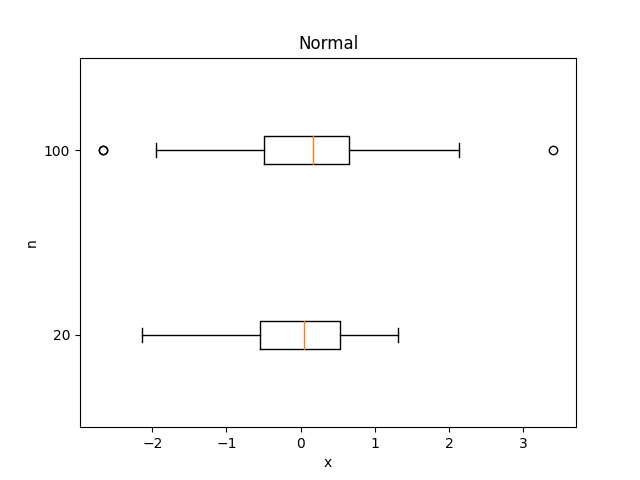
\includegraphics[scale=0.65]{normal_boxplot.png}
	\caption{Боксплот нормального распределения}
\end{figure}

\begin{figure}[H]
	\centering
	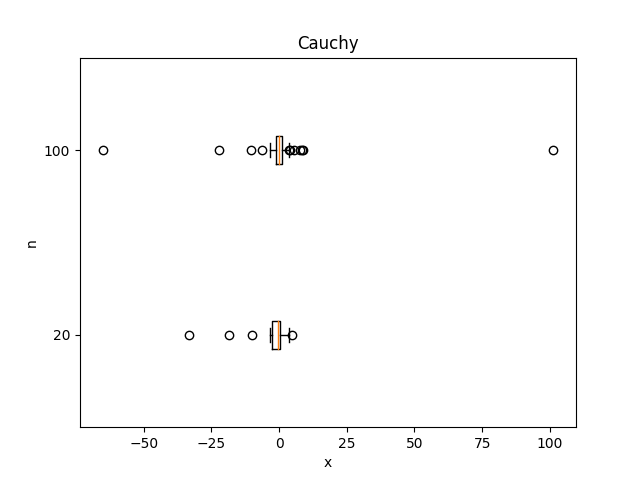
\includegraphics[scale=0.65]{cauchy_boxplot.png}
	\caption{Боксплот распределения Коши}
\end{figure}

\begin{figure}[H]
	\centering
	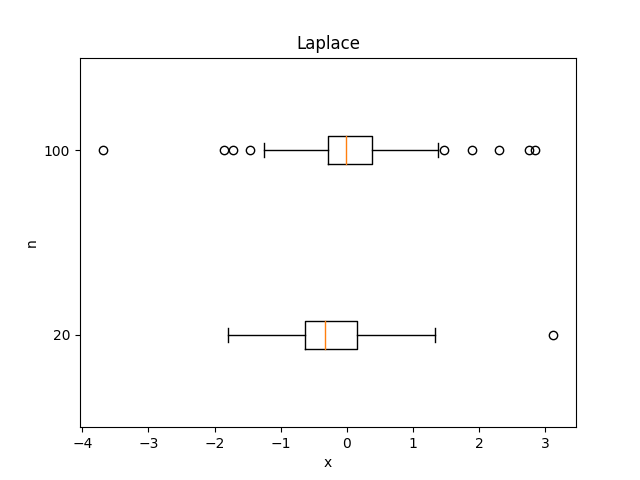
\includegraphics[scale=0.65]{laplace_boxplot.png}
	\caption{Боксплот распределения Лапласа}
\end{figure}

\begin{figure}[H]
	\centering
	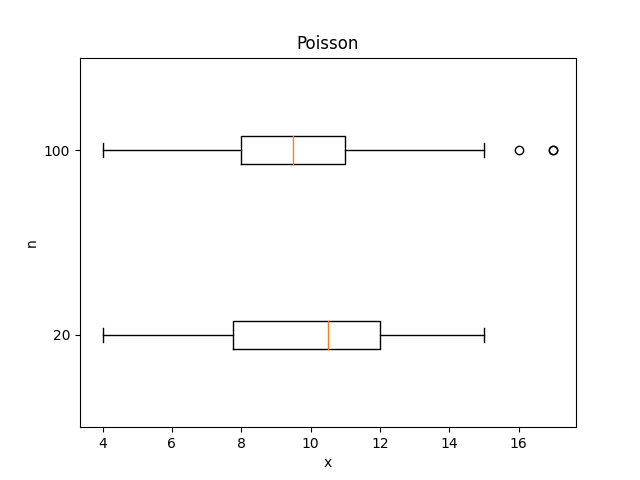
\includegraphics[scale=0.65]{poisson_boxplot.png}
	\caption{Боксплот распределения Пуассона}
\end{figure}

\begin{figure}[H]
	\centering
	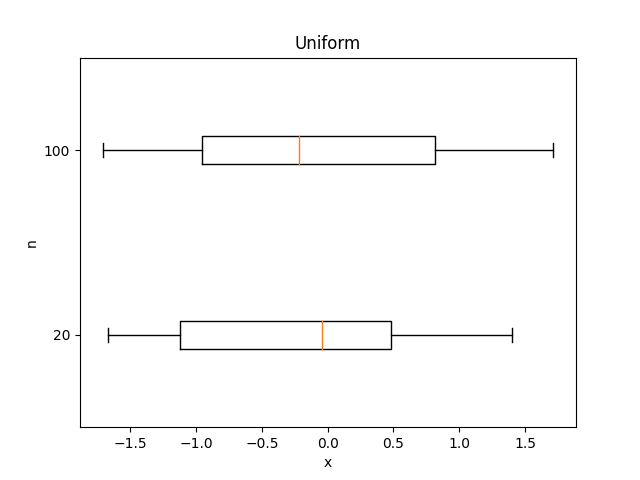
\includegraphics[scale=0.65]{uniform_boxplot.png}
	\caption{Боксплот равномерного распределения}
\end{figure}

\subsection{Доля выбросов}

Округление осуществлялось следующим образом: \\
Выборка случайна, поэтому в качестве оценки рассеяния можно взять дисперсию пуассоновского потока: $D_{n} \approx \sqrt{n}$ \\
Доля $p_n = \dfrac{D_n}{n}=\dfrac{1}{\sqrt{n}} $ \\
Для n=20: $p_n = \dfrac{1}{\sqrt{20}}$ -- примерно 0.2 или 20 \% \\
Для n=100 $p_n = 0.1$ или 10 \% \\
Исходя из этого можно решить, сколько знаков оставлять в доле выбросов\\
\begin{table}[H]
	\begin{center}
		\begin{tabular}{|c|c|}
			\hline
			Выборка & Доля выбросов \\
			\hline\hline
			Normal n=20 & 0.02\\
			\hline 
			Normal n=100 & 0.01\\
			\hline
			Cauchy n=20 & 0.15\\
			\hline 
			Cauchy n=100 & 0.15\\
			\hline
			Laplace n=20 & 0.07\\
			\hline 
			Laplace n=100 & 0.06\\
			\hline
			Poisson n=20 & 0.02\\
			\hline 
			Poisson n=100 & 0.01\\
			\hline
			Uniform n=20 & 0.00\\
			\hline 
			Uniform n=100 & 0.00\\
			\hline
		\end{tabular}
	\end{center}
    \caption{Доля выбросов}
\end{table}




\subsection{Теоретическая вероятность выбросов}

\begin{table}[H]
	\begin{center}
		\begin{tabular}{|c|c|c|c|c|c|}
			\hline 
			Распределение & $Q_{1}^{T}$ & $Q_{3}^{T}$ & $X_{1}^{T}$ & $X_{2}^{T}$ & $P_{B}^{T}$ \\
			\hline\hline 
			 Нормальное распределение & -0.674 & 0.674  & -2.698  & 2.698 & 0.007\\
			\hline
			 Распределение Коши & -1 & 1 &-4  &4 &0.156\\
			\hline
			 Распределение Лапласа & -0.490 & 0.490 &-1.961  &1.961 &0.063\\
			\hline
			 Распределение Пуассона &8 &12  &2  &18 & 0.008 \\
			\hline
			 Равномерное распределение &-0.866 &0.866  &-3.464  &3.464 &0\\
			\hline
		\end{tabular}
	\end{center}
    \caption{Теоретическая вероятность выбросов}
\end{table}

\subsection{Эмпирическая функция распределения}

Графики теоретической функции распределения синего цвета, графики эмперической функции распределения -- черного. \\

\begin{figure}[H]
	\begin{tabular}{ccc}
		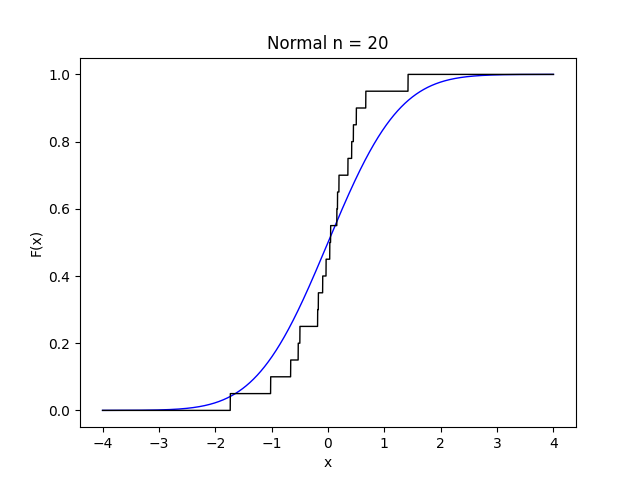
\includegraphics[scale=0.33]{normal_F20.png}
		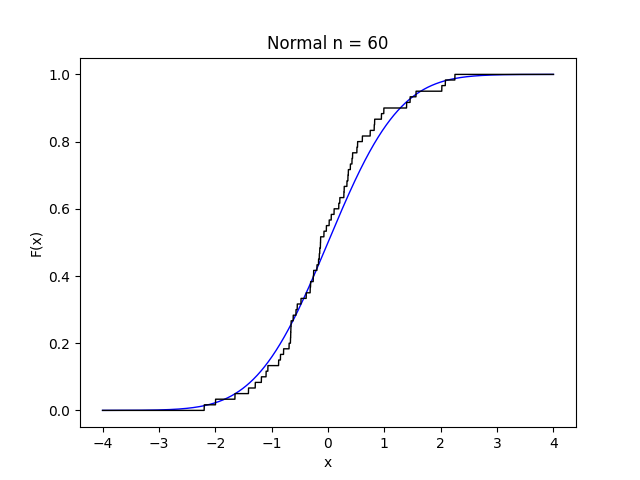
\includegraphics[scale=0.33]{normal_F60.png}
		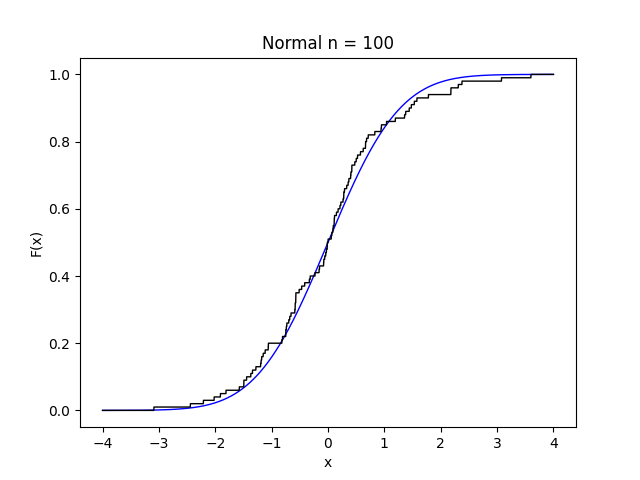
\includegraphics[scale=0.33]{normal_F100.png}
	\end{tabular}
	\caption{Функция распределения вероятности нормального р-я}
\end{figure}

\begin{figure}[H]
	\begin{tabular}{ccc}
		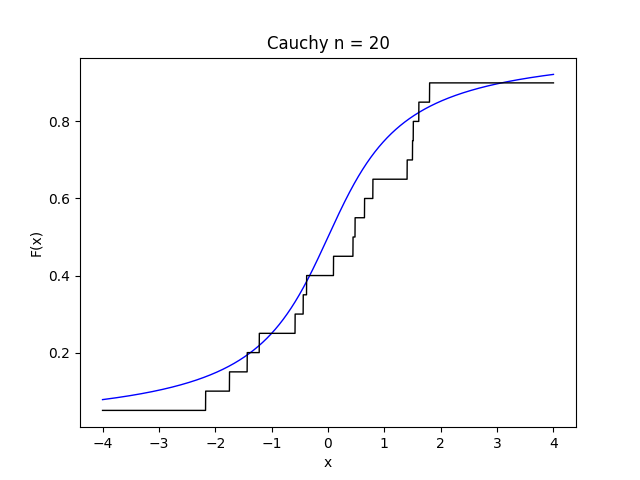
\includegraphics[scale=0.33]{cauchy_F20.png}
		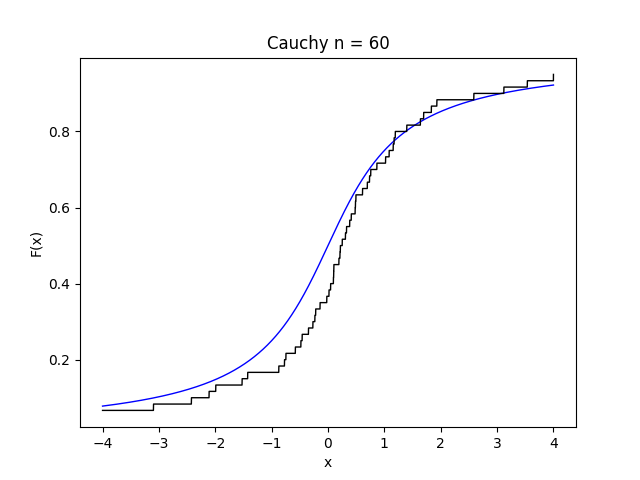
\includegraphics[scale=0.33]{cauchy_F60.png}
		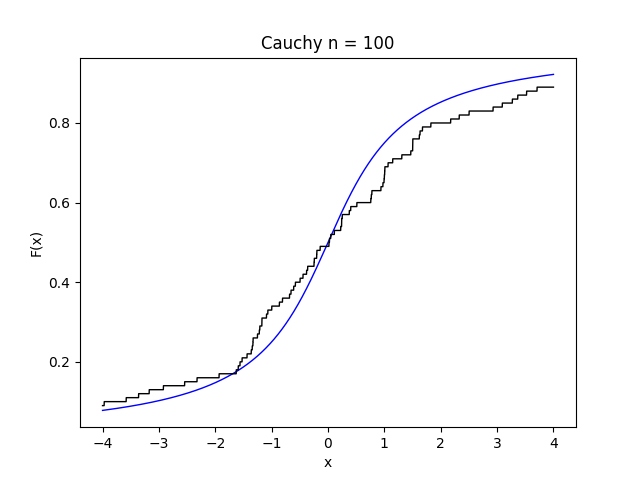
\includegraphics[scale=0.33]{cauchy_F100.png}
	\end{tabular}
	\caption{Функция распределения вероятности р-я Коши}
\end{figure}

\begin{figure}[H]
	\begin{tabular}{ccc}
		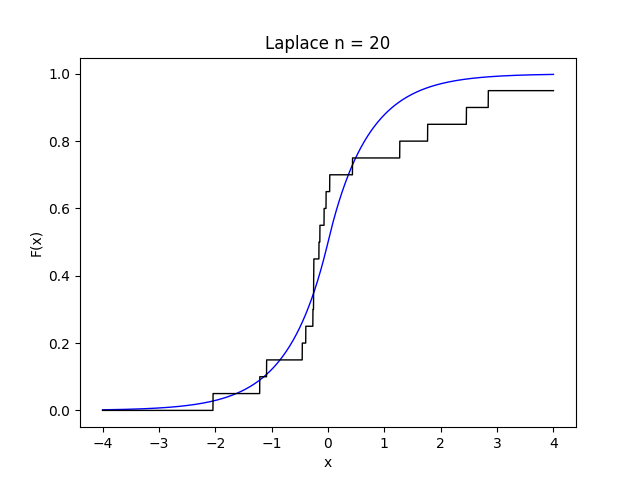
\includegraphics[scale=0.33]{laplace_F20.png}
		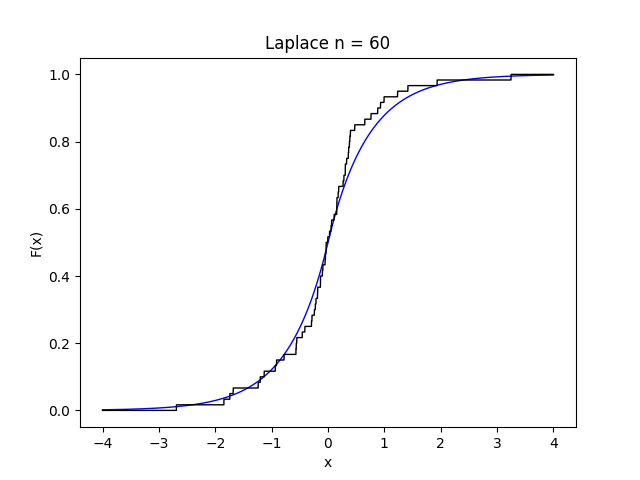
\includegraphics[scale=0.33]{laplace_F60.png}
		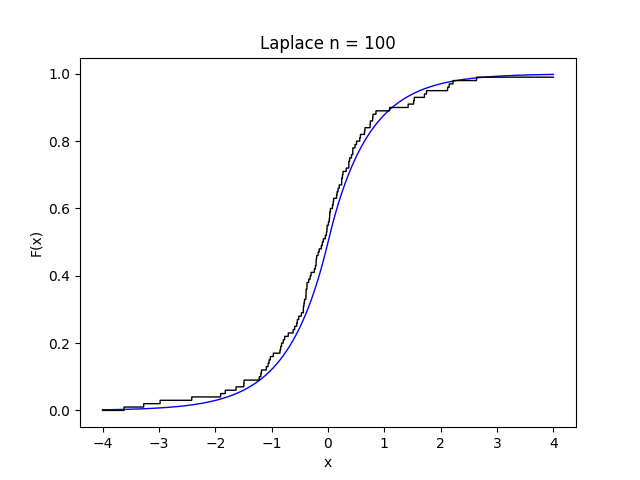
\includegraphics[scale=0.33]{laplace_F100.png}
	\end{tabular}
	\caption{Функция распределения вероятности р-я Лапласа }
\end{figure}

\begin{figure}[H]
	\begin{tabular}{ccc}
		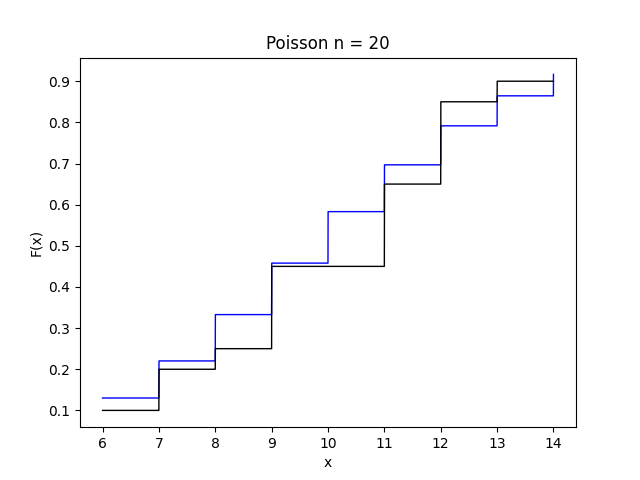
\includegraphics[scale=0.33]{poisson_F20.png}
		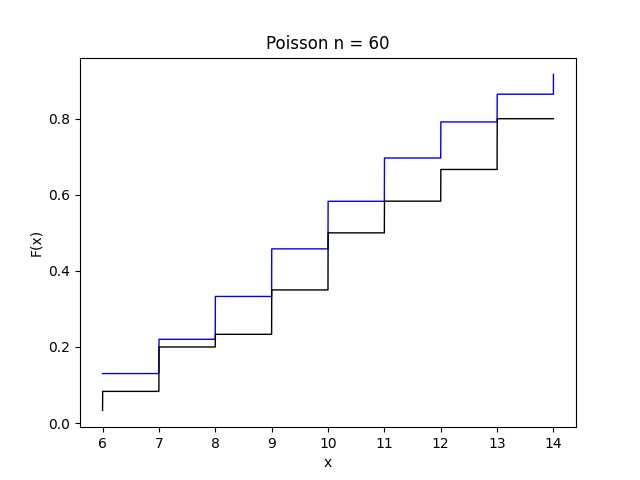
\includegraphics[scale=0.33]{poisson_F60.png}
		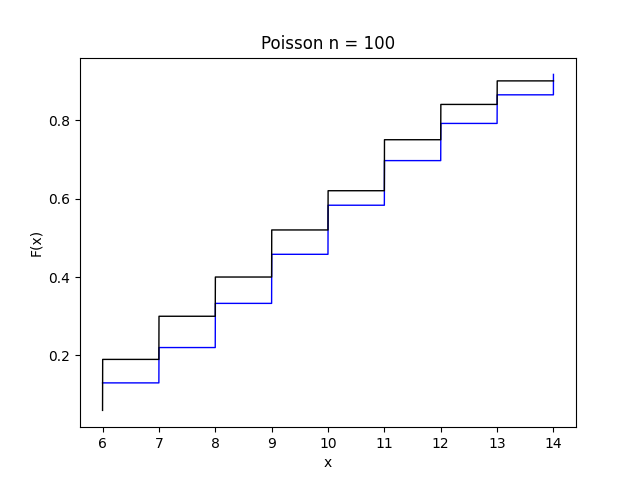
\includegraphics[scale=0.33]{poisson_F100.png}
	\end{tabular}
	\caption{Функция распределения вероятности р-я Пуассона}
\end{figure}


\begin{figure}[H]
	\begin{tabular}{ccc}
		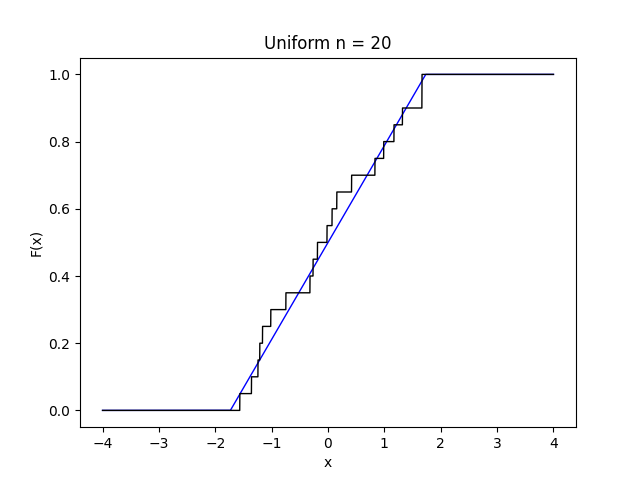
\includegraphics[scale=0.33]{uniform_F20.png}
		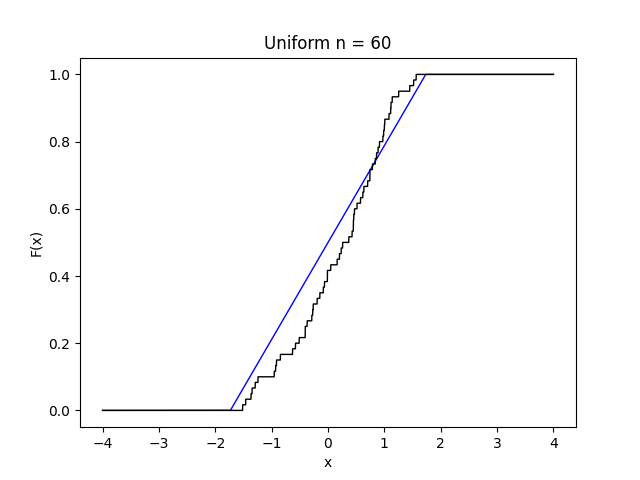
\includegraphics[scale=0.33]{uniform_F60.png}
		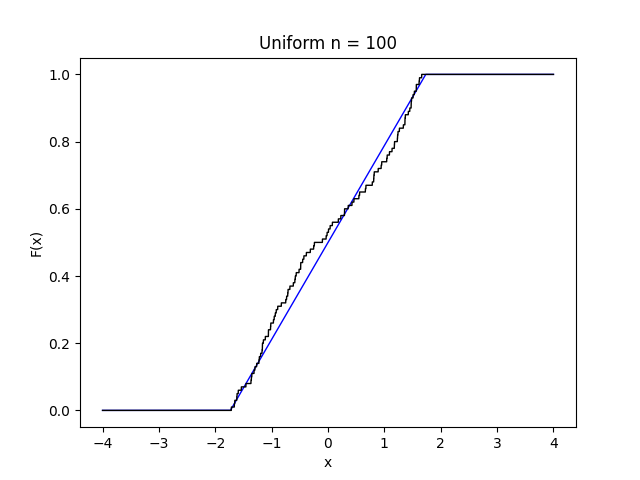
\includegraphics[scale=0.33]{uniform_F100.png}
	\end{tabular}
	\caption{Функция распределения вероятности равномерного р-я}
\end{figure}

\subsection{Ядерные оценки плотности распределения}

Графики плотности распределения красного цвета, графики оценок -- черного. \\
$adjust = 0.5$ соответствует $h = \dfrac{h_{n}}{2}$ \\
$adjust = 1$ соответствует $h = h_{n}$ \\
$adjust = 2$ соответствует $h = 2h_{n}$ \\

\begin{figure}[H]
	\begin{tabular}{ccc}
		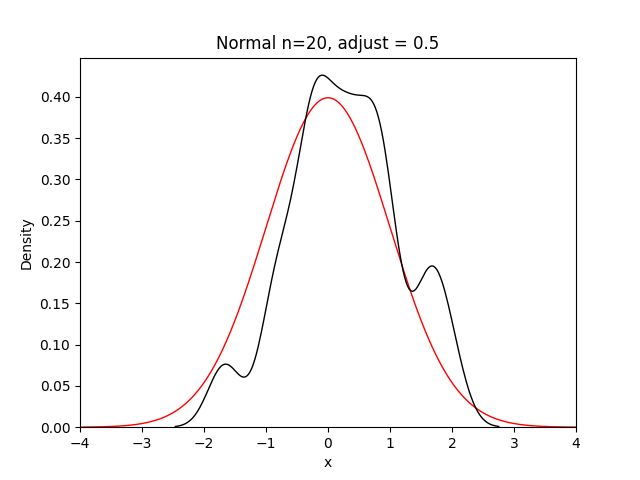
\includegraphics[scale=0.33]{normal_n20_adjust0.5.png}
		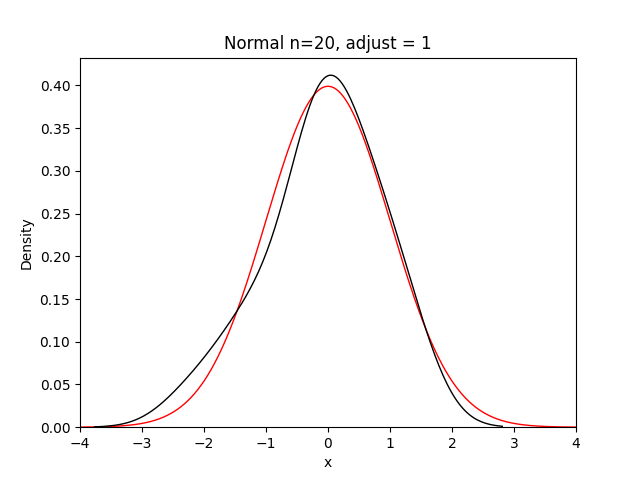
\includegraphics[scale=0.33]{normal_n20_adjust1.png}
		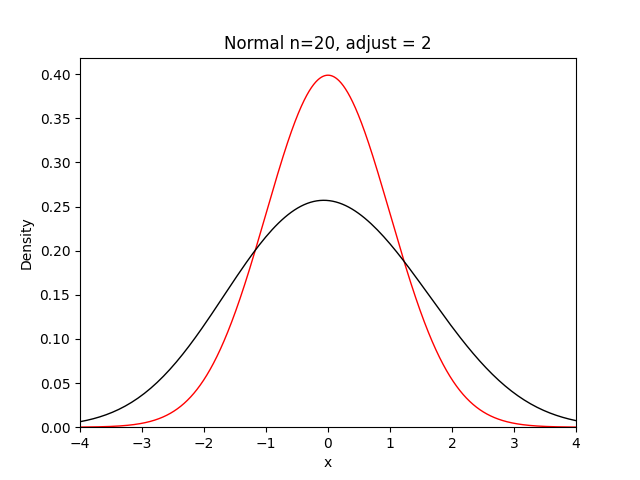
\includegraphics[scale=0.33]{normal_n20_adjust2.png}
	\end{tabular}
	\caption{Нормальное распределение, n=20}
\end{figure}

\begin{figure}[H]
	\begin{tabular}{ccc}
		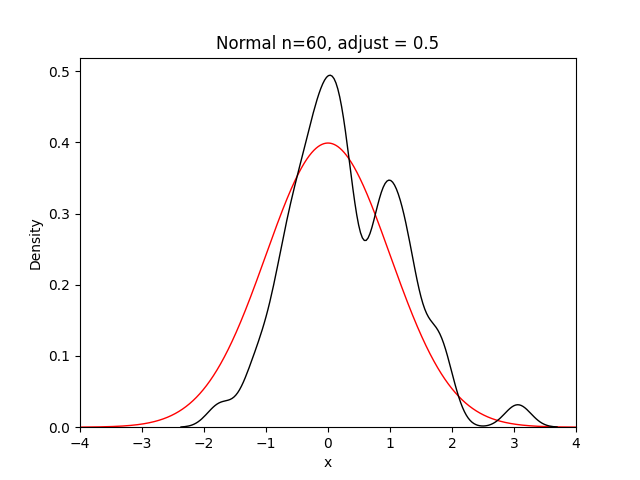
\includegraphics[scale=0.33]{normal_n60_adjust0.5.png}
		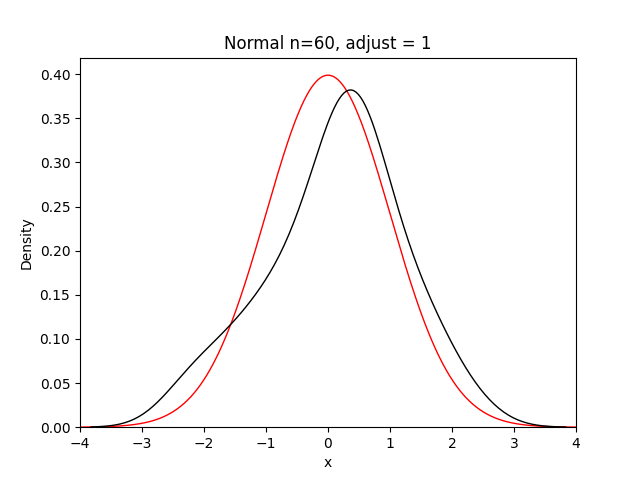
\includegraphics[scale=0.33]{normal_n60_adjust1.png}
		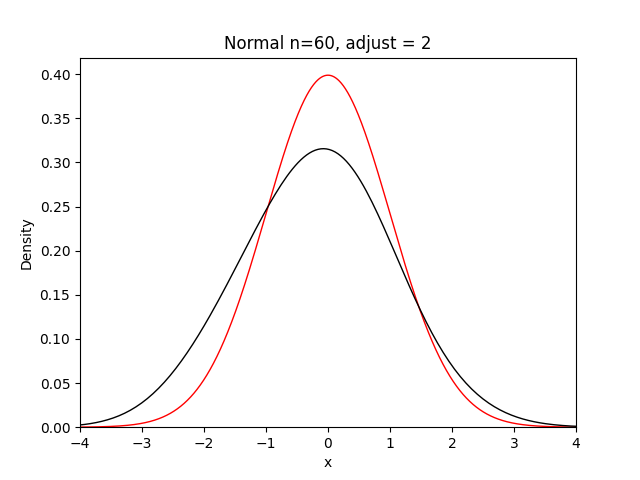
\includegraphics[scale=0.33]{normal_n60_adjust2.png}
	\end{tabular}
	\caption{Нормальное распределение, n=20}
\end{figure}

\begin{figure}[H]
	\begin{tabular}{ccc}
		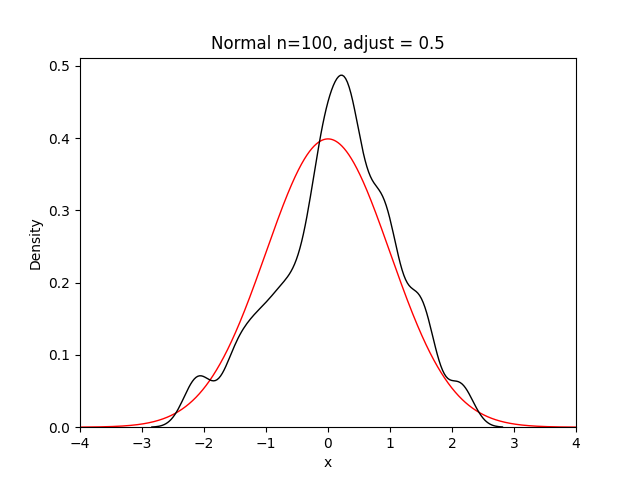
\includegraphics[scale=0.33]{normal_n100_adjust0.5.png}
		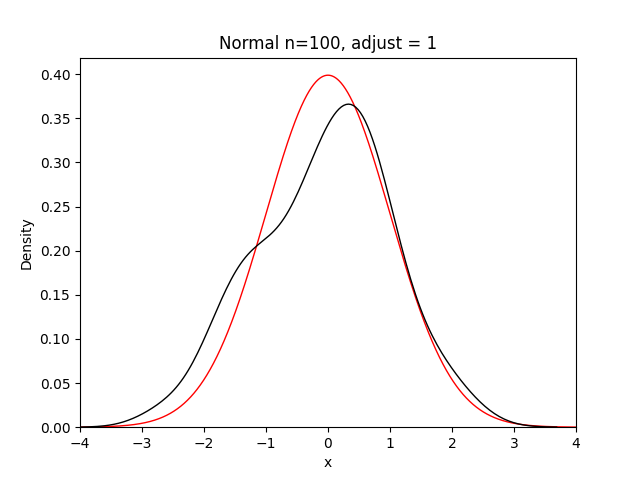
\includegraphics[scale=0.33]{normal_n100_adjust1.png}
		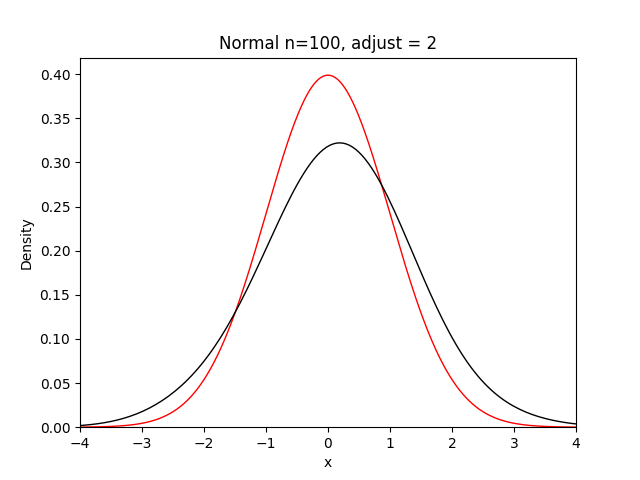
\includegraphics[scale=0.33]{normal_n100_adjust2.png}
	\end{tabular}
	\caption{Нормальное распределение, n=100}
\end{figure}


\begin{figure}[H]
	\begin{tabular}{ccc}
		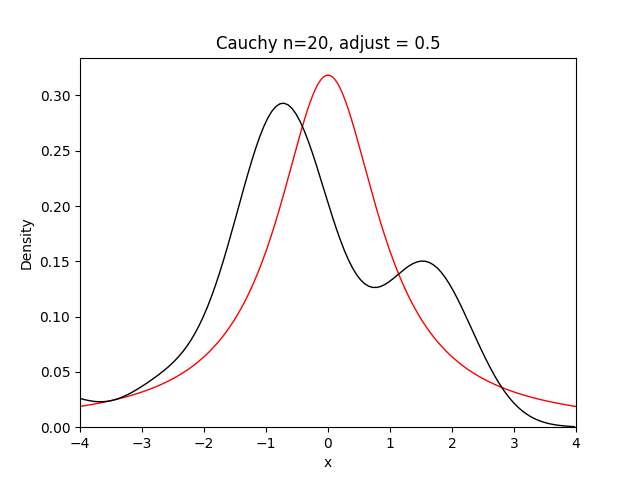
\includegraphics[scale=0.33]{cauchy_n20_adjust0.5.png}
		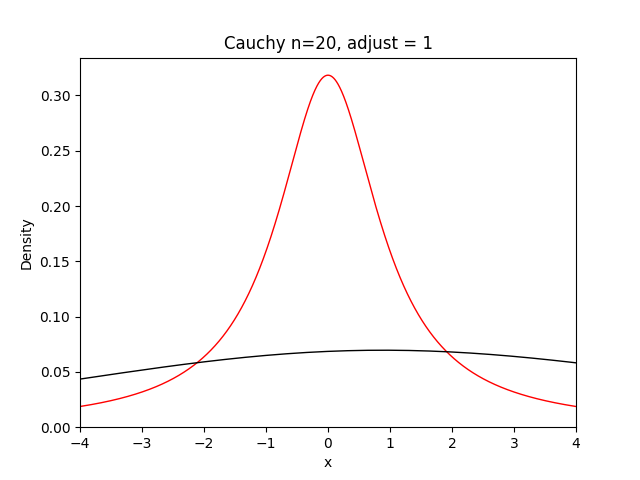
\includegraphics[scale=0.33]{cauchy_n20_adjust1.png}
		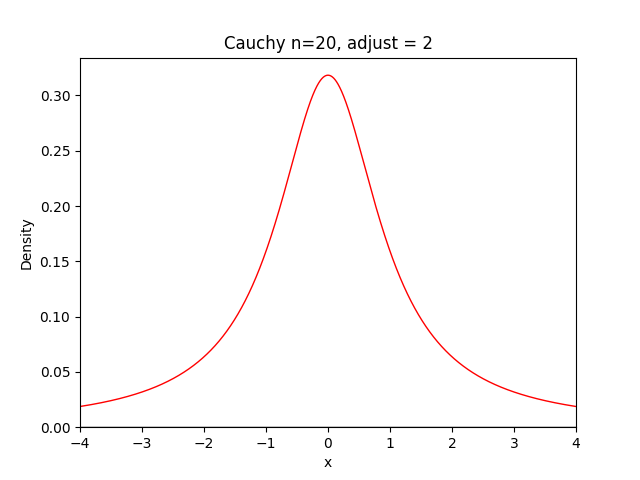
\includegraphics[scale=0.33]{cauchy_n20_adjust2.png}
	\end{tabular}
	\caption{Распределение Коши, n=20}
\end{figure}

\begin{figure}[H]
	\begin{tabular}{ccc}
		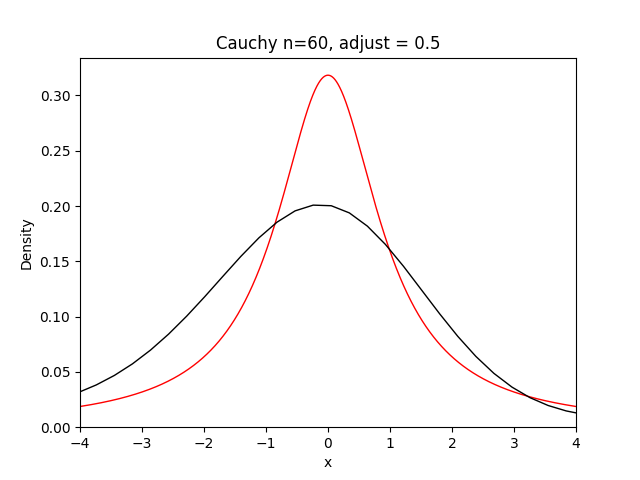
\includegraphics[scale=0.33]{cauchy_n60_adjust0.5.png}
		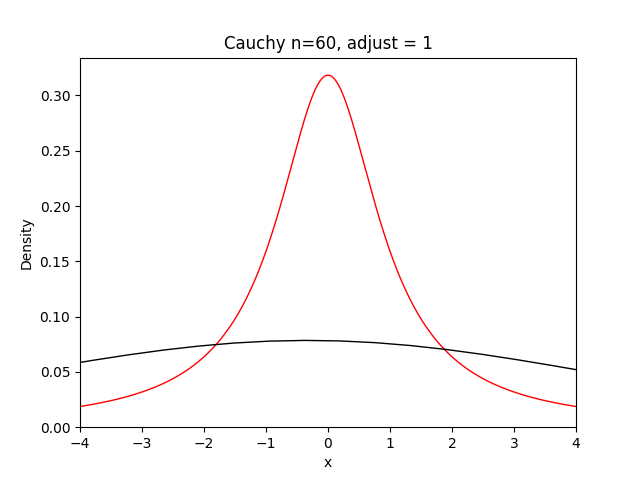
\includegraphics[scale=0.33]{cauchy_n60_adjust1.png}
		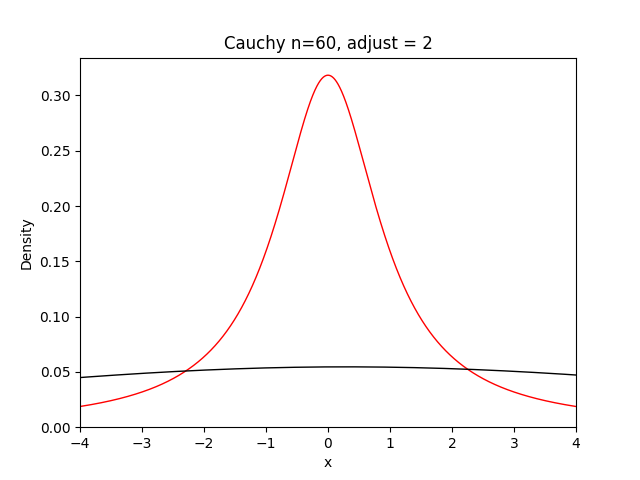
\includegraphics[scale=0.33]{cauchy_n60_adjust2.png}
	\end{tabular}
	\caption{Распределение Коши, n=60}
\end{figure}

\begin{figure}[H]
	\begin{tabular}{ccc}
		\includegraphics[scale=0.33]{cauchy_n100_adjust0.5.png}
		\includegraphics[scale=0.33]{cauchy_n100_adjust1.png}
		\includegraphics[scale=0.33]{cauchy_n100_adjust2.png}
	\end{tabular}
	\caption{Распределение Коши, n=100}
\end{figure}

\begin{figure}[H]
	\begin{tabular}{ccc}
		\includegraphics[scale=0.33]{laplace_n20_adjust0.5.png}
		\includegraphics[scale=0.33]{laplace_n20_adjust1.png}
		\includegraphics[scale=0.33]{laplace_n20_adjust2.png}
	\end{tabular}
	\caption{Распределение Лапласа, n=20}
\end{figure}

\begin{figure}[H]
	\begin{tabular}{ccc}
		\includegraphics[scale=0.33]{laplace_n60_adjust0.5.png} 
		\includegraphics[scale=0.33]{laplace_n60_adjust1.png}
		\includegraphics[scale=0.33]{laplace_n60_adjust2.png}
	\end{tabular}
	\caption{Распределение Лапласа, n=60}
\end{figure}

\begin{figure}[H]
	\begin{tabular}{ccc}
		\includegraphics[scale=0.33]{laplace_n100_adjust0.5.png}
		\includegraphics[scale=0.33]{laplace_n100_adjust1.png}
		\includegraphics[scale=0.33]{laplace_n100_adjust2.png}
	\end{tabular}
	\caption{Распределение Лапласа, n=100}
\end{figure}

\begin{figure}[H]
	\begin{tabular}{ccc}
		\includegraphics[scale=0.33]{poisson_n20_adjust0.5.png}
		\includegraphics[scale=0.33]{poisson_n20_adjust1.png}
		\includegraphics[scale=0.33]{poisson_n20_adjust2.png}
	\end{tabular}
	\caption{Распределение Пуассона, n=20}
\end{figure}

\begin{figure}[H]
	\begin{tabular}{ccc}
		\includegraphics[scale=0.33]{poisson_n60_adjust0.5.png}
		\includegraphics[scale=0.33]{poisson_n60_adjust1.png}
		\includegraphics[scale=0.33]{poisson_n60_adjust2.png}
	\end{tabular}
	\caption{Распределение Пуассона, n=60}
\end{figure}

\begin{figure}[H]
	\begin{tabular}{ccc}
		\includegraphics[scale=0.33]{poisson_n100_adjust0.5.png}
		\includegraphics[scale=0.33]{poisson_n100_adjust1.png}
		\includegraphics[scale=0.33]{poisson_n100_adjust2.png}
	\end{tabular}
	\caption{Распределение Пуассона, n=100}
\end{figure}


\begin{figure}[H]
	\begin{tabular}{ccc}
		\includegraphics[scale=0.33]{uniform_n20_adjust0.5.png}
		\includegraphics[scale=0.33]{uniform_n20_adjust1.png}
		\includegraphics[scale=0.33]{uniform_n20_adjust2.png}
	\end{tabular}
	\caption{Равномерное распределение, n=20}
\end{figure}

\begin{figure}[H]
	\begin{tabular}{ccc}
		\includegraphics[scale=0.33]{uniform_n60_adjust0.5.png}
		\includegraphics[scale=0.33]{uniform_n60_adjust1.png}
		\includegraphics[scale=0.33]{uniform_n60_adjust2.png}
	\end{tabular}
	\caption{Равномерное распределение, n=60}
\end{figure}

\begin{figure}[H]
	\begin{tabular}{ccc}
		\includegraphics[scale=0.33]{uniform_n100_adjust0.5.png}
		\includegraphics[scale=0.33]{uniform_n100_adjust1.png}
		\includegraphics[scale=0.33]{uniform_n100_adjust2.png}
	\end{tabular}
	\caption{Равномерное распределение, n=100}
\end{figure}


